
\section{Start met de BBC microbit}

De BBC Microbit is ontwikkeld om programmeeronderwijs te kunnen geven aan leerlingen van groep 7 (10/11-jarigen). Sinds 2016 wordt dit bordje aan elke groep 7 leerling verstrekt, elk jaar ongeveer 1 miljoen stuks. De hardware, het bordje is ‘open source’, de software die we er bij gebruiken ook.

De hardware is robuust, goedkoop, héél eenvoudig te programmeren, je kunt er veel mee en er is prima ondersteuning. Er zijn verschillende ontwikkel omgevingen gebruiken om programma’s te schrijven voor de Microbit. 

Je gaat de Microbit gebruiken in ‘The Challenge’. De Microbit is een Embedded System. Een Embedded System bestaat uit een microcontroller met sensoren en actuatoren. Met sensoren meet je iets (licht, temperatuur, beweging), met actuatoren stuur je iets aan (b.v een ledje, een speakertje, een motor, etc.). Met de Microbit kun je IoT (Internet of Things) devices simuleren, dit zijn ook Embedded Systems. Met een IoT device wordt meestal een apparaat bedoeld die een radiomodule bevat die data kan verzenden of ontvangen. Je kunt deze radiomodule zien als een black box. Er zijn veel verschillende typen voor veel verschillende toepassingen. Ze verschillen in bereik, datadoorvoer, reactiesnelheid en energieverbruik. 
Voor ‘The Challenge’ maakt het niet uit, je kunt met de Microbit prima een IoT device simuleren.

Let op: Het installeren van software moet je zelf uitzoeken, dit kost veel tijd. Verwacht daarom niet dat je docent je hiermee kan helpen!

Indien het niet lukt, kan altijd om hulp gevraagd worden, maar doe dat met specifieke vragen en vertelt erbij wat jezelf al uitgeprobeerd heb.

\subsection{Eerste kennismaking met de Microbit}

Sluit de microbit met behulp van een USB micro snoertje aan op je laptop, zoals te zien is in figuur \ref{fig:aansluiting}.
Windows herkent de microbit en kent daar een \textbf{drive letter} voor, zoals ook gebeurt bij een USB stick. Dit is te zien in figuur \ref{fig:driveL}.


\begin{figure}[h!]
	\captionsetup{justification=centering}
	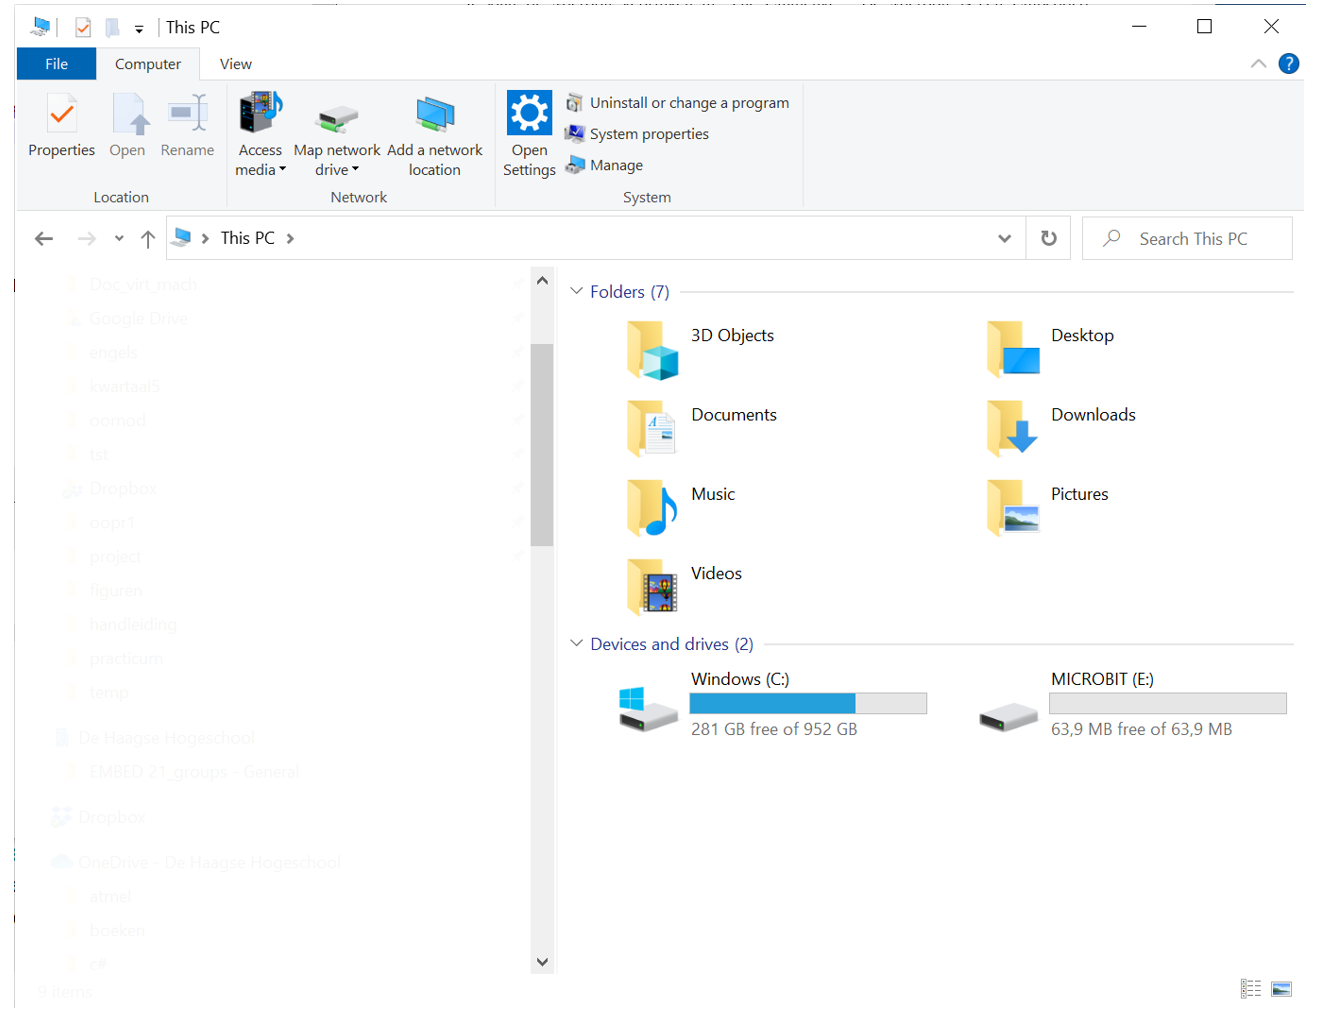
\includegraphics[width=0.50 \linewidth]{figuren/driverLetter}
	\centering
	\caption{Herkenning microbit in windows.}
	\label{fig:driveL}
\end{figure}

Na het aansluiten zal bij een nieuwe BBC microbit de ingebouwde demo gaan lopen. Werkt de ingebouwde demo niet, dan kan je naar de \href{https://support.microbit.org/support/solutions/articles/19000021613-reset-the-micro-bit-to-factory-defaults}{Reset de micro:bit to factory pagina} gaan en download het  \href{https://support.microbit.org/helpdesk/attachments/19067609189} {OutOfBoxExperience.hex} programma en zet dit op de MICROBIT drive. Hierdoor zal het programma geüpload worden op de microbit.

Voor verdere kennismaking met de microbit is de de pagina \href{https://microbit.org/get-started/first-steps/set-up/}{https://microbit.org/get-started/first-steps/set-up/}
een goed startpunt.


\subsection{De Microbit in “The Challenge”}

De doelstelling van The Challenge is dat hier producten van alle differentiaties in samenkomen. Voor het NSE/Embedded deel houden we het eenvoudig.


Je zou tijdens de Challenge eventueel ook de microbit met \href{https://docs.arduino.cc/micropython/?_gl=1*bbja8p*_gcl_au*MTA0MzMyMzUwNC4xNzI4NDYwNDQ0*FPAU*MTA0MzMyMzUwNC4xNzI4NDYwNDQ0*_ga*MTM2NDc5NzM2OC4xNzI4NDYwNDQy*_ga_NEXN8H46L5*MTcyODQ2MDQ0MS4xLjEuMTcyODQ2MDQ5MS4wLjAuMTk3NzAxMDU1NQ..*_fplc*dmdpUTJCaSUyQjFINjd2SExxV092Zml5Ym92VlZQMGdtNWFSeG0lMkJLWEpQSnFDMkE4cG52M1klMkJGcGdNYzRKNGhBTkMzRXcyOXc0Ykhvcndmc0UyMVdwM1U2Rzc0bkFURWoxRHBWN3RlbjNvMlRNOVJ0eW1nSmp3OXFucURhWW9BJTNEJTNE}{micropython} kunnen programmeren.
Verder is er nog een mogelijkheid om de “blokken” taal te gebruiken. Hier kun je ook alles mee.
Voor een intro in de “blokken” taal, start hier en begin met ‘Mode’, ‘Step Counter’, kies voor ‘Instructies weergeven’: \href{https://makecode.microbit.org/}{https://makecode.microbit.org/}

Het ligt voor de hand dat NSE studenten in de Arduino omgeving programmeren, waar de programmeertalen C/C++ de voertaal is.\\